\documentclass{article}
%%%%%%%%%%%%%%%%%%%%%%%%%%%%%%%%%%%%%%%%%%%%%%%%%%%%%%%%%%%%%%%%%%%%%%%%%%%%%%%
% PREAMBLE
%%%%%%%%%%%%%%%%%%%%%%%%%%%%%%%%%%%%%%%%%%%%%%%%%%%%%%%%%%%%%%%%%%%%%%%%%%%%%%%
\usepackage{mathtools}
\usepackage{algorithm}
\usepackage{algorithmic}
\usepackage{fancyvrb}
\usepackage{booktabs}
\usepackage{rotating}
\usepackage{tikz}
\usepackage{float}
\usepackage{hyperref}
\usepackage{subcaption}
\usetikzlibrary{arrows,decorations.pathmorphing,backgrounds,positioning,fit,matrix}
\newcommand{\DepProps}{\textsc{DepProps}}
\usepackage{titling}
\newcommand{\subtitle}[1]{%
  \posttitle{%
    \par\end{center}
    \begin{center}\large#1\end{center}
    \vskip0.5em}%
}
\begin{document}
% TITLE
\title{DM819 - Computational Geometry}
\subtitle{Fall 2015\\Project 2}
% AUTHER
\author{Mikkel Levisen and Jesper Lund}
%DATE
\maketitle
% no page number on first page
\thispagestyle{empty}
\newpage
% TABLE OF CONTENTS
\tableofcontents
% no page number on table of contents page
\thispagestyle{empty}
\newpage
% restart page number counter
\pagenumbering{arabic} 
%%%%%%%%%%%%%%%%%%%%%%%%%%%%%%%%%%%%%%%%%%%%%%%%%%%%%%%%%%%%%%%%%%%%%%%%%%%%%%%
% DOCUMENT START
%%%%%%%%%%%%%%%%%%%%%%%%%%%%%%%%%%%%%%%%%%%%%%%%%%%%%%%%%%%%%%%%%%%%%%%%%%%%%%%
\section{Introduction}
  This report details the implementation of KD-Tree and Range-Tree for 
  $d$-dimensional input. Each tree is constructed from a list of unsorted points
  and is capable of performing orthogonal range queries.
  \subsection{Definitions}
  \begin{itemize}
  	\item a $d$-dimensional point, $p$, consists of real numbers $(p_1,p_2,\dots,p_d)$
  	\item a $d$-dimensional range, $R$, is a hyper-volume defined by $[r_1:r_1']
  	\times[r_2:r_2']\times \dots \times [r_d:r_d']$, where each $r$ is a real number
  \end{itemize}

  \subsection{Range Queries}
  Given a set of points, $P$, and a range object, $R$, a range query consist of
  reporting all points in $P$ which intersect $R$ e.g. a 1-dimensional point
  set $\{1,2,3,4,5\}$ and a range object $[2:4]$ yields $\{2,3,4\}$. 
  
  
  
  %that intersects 
  %a 
  %A point $p \in P$ exists in the range $R$ iff.
  %\[
  %  \forall p_i \in p: \{ R_{i,1}\leq   p_i \leq R_{i,2}\}|\forall i \in \{1,...,n\}, n = dimensions 
  %\]
  %
  %A range query consists of reporting all points, $p$, which lie within a given 
  %range, $R$.
  %An $n$-dimensional point, $P_n$, consist of real numbers 
  %$\{p_1,p_2,\dots,p_n\}$, and an $n$-dimensional range $R_n$ consist of 
  %$[x:x']\times[y:y'] \times \dots \times[z:z']$. A range query consist of 
  %reporting all points $P_n$ in a range $R_n$.
\section{KD-Tree}
\subsection{Complexity}
\section{Range-Tree}
  A Range-tree is a multi-level data structure for time efficient range queries.
  In 2-dimensional the firs-level of the range tree is a binary search tree on 
  the $x$-coordinate. Each node has an associated data structure for all
  points in its canonical set. The associated data structure is a binary 
  search tree on the $y$-coordinate of the points. 
  To report which points are in a given range is a 1-dimensional range search 
  performed for each dimension, that is, first find all leaf nodes which lie 
  within $[x:x']$ in the first level, then determine which of those nodes 
  $y$-coordinate lie within $[y:y']$ on the second level. 
 \section{Test}
    \subsection{Test Generation}
    Supplied with the code is a test generating script which can create tests of
    arbitrary dimension and size. The tests are stored in directories by 
    dimension.
    
    In a tests consisting of $n$ points in $d$ dimensions a $d$-dimensional 
    volume is constructed with a side length $s = \sqrt[d]{n}$. For each such 
    volume is $1000$ ranges generated with a side length of 
    $rs = \sqrt[d]{0.1 \cdot s^d}$ i.e. each range will contain approximately 
    10\% of the $n$ points. 
\begin{figure}[H]
    \centering
    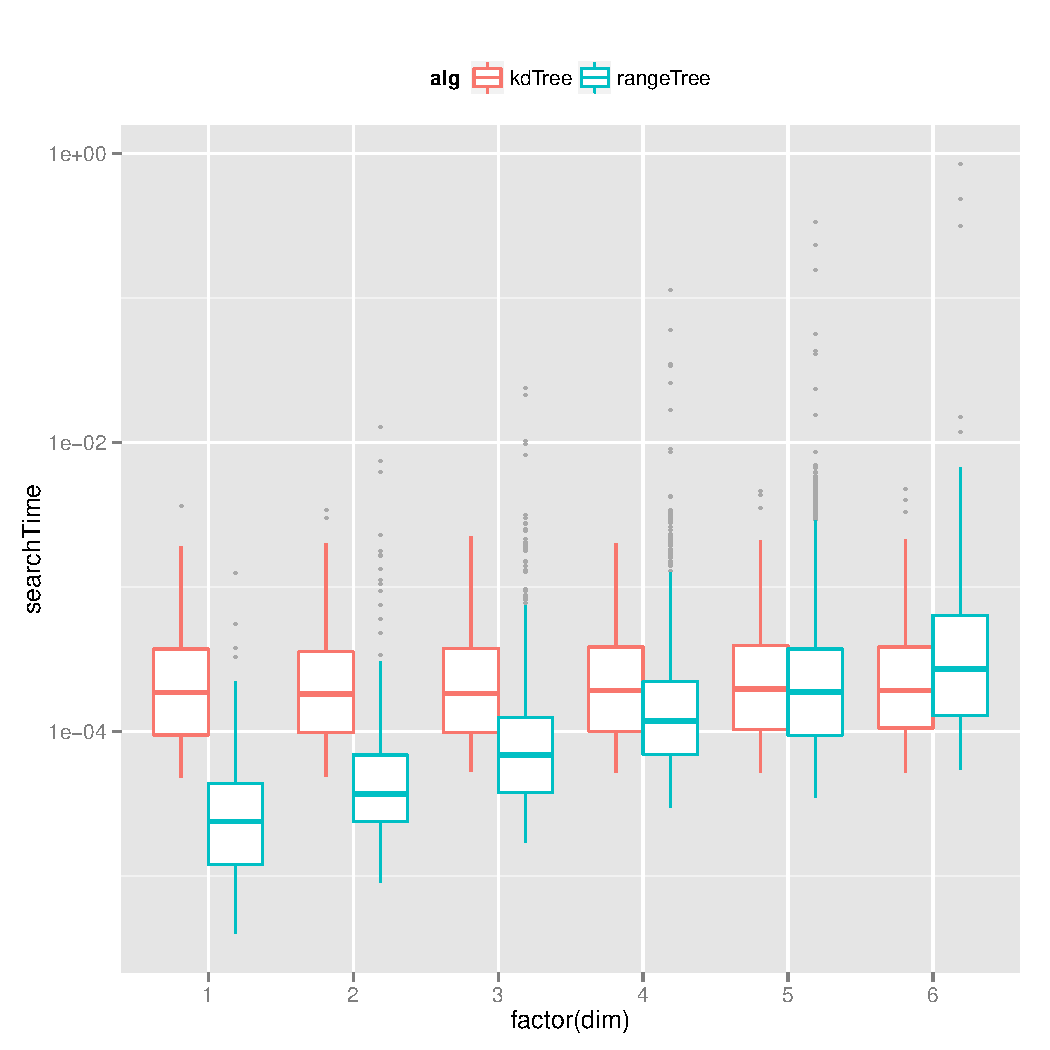
\includegraphics[width=\textwidth]{../src/R/plots/boxplot.pdf}
\end{figure}
\begin{figure}[H]
    \centering
    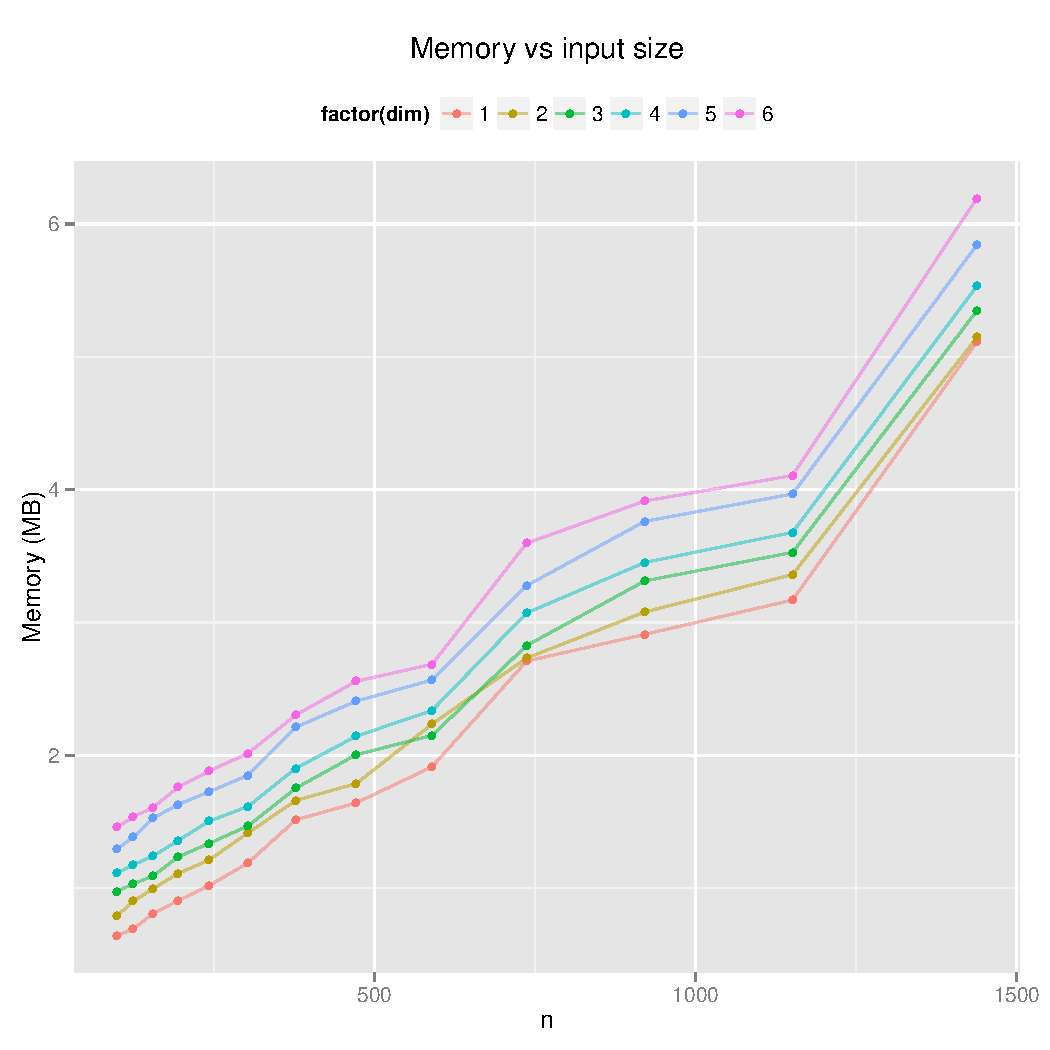
\includegraphics[width=\textwidth]{../src/R/plots/kdmem.pdf}
\end{figure}
\begin{figure}[H]
    \centering
    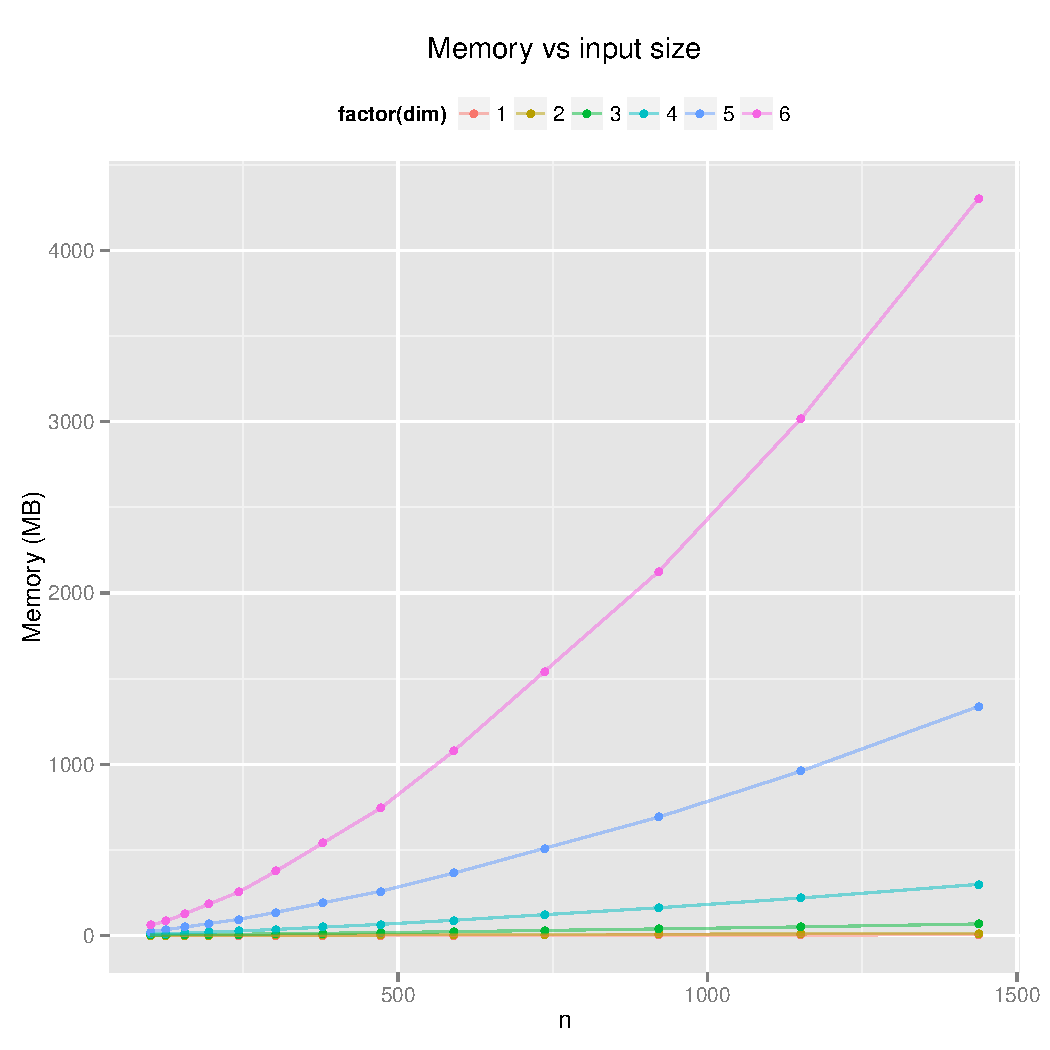
\includegraphics[width=\textwidth]{../src/R/plots/rtmem.pdf}
\end{figure}
\section{Manual}
  \subsection{File Formats}
  \subsubsection{Input}
  The input file format consist of two distinctest parts: \textit{points} and 
  \textit{ranges}. 
  \\
  \\
  Points are real numbers separated by \verb|<TAB>|. 
  \begin{verbatim}
  	<real> \t <real>
  	<real>:<real> \t <real>:<real> [, <integer> \t <integer>]
  \end{verbatim}

  \subsection{Inscrutions}
\subsection{File Structure}
\begin{verbatim}
ROOT
|-- report/
`-- src
    |-- kdtree
    |   |-- inspect.lua
    |   |-- kdtree.lua
    |   `-- test.lua
    |-- R
    |   `-- makePlots.R
    |-- rangeTree
    |   |-- inspect.lua
    |   |-- middleclass
    |   |   `-- middleclass.lua
    |   |-- RangeTree.lua
    |   `-- test.lua
    |-- results/
    |-- runTests.py
    `-- tests
        |-- createCustomTest.lua
        |-- dimension_1/
        |-- dimension_2/
        |-- dimension_3/
        |-- dimension_4/
        |-- dimension_5/
        |-- dimension_6/
        |-- genTestSuite.lua
        `-- inspect.lua
\end{verbatim}

\section{Conclusion}
\end{document}